% !TeX root = main.tex
\chapter{Gemmini's Internal Architecture and Programming Model}
\label{chap:gemmini_internals}

While Chapter \ref{chap:gemmini_overview} described the conceptual architecture of \texttt{Gemmini}, this chapter explores its internal structure and the software interfaces used to control it. A deeper understanding of these implementation-level details is necessary to effectively program the accelerator and analyze its performance.

\section{Internal Command and Control Flow}
\label{sec:gemmini_internal_flow}

A custom \texttt{RoCC} instruction sent from the \texttt{Rocket} core is not executed directly by the systolic array. Instead, it triggers a complex sequence of events within the \texttt{Gemmini} accelerator's internal controller modules. The overall structure of the generated hardware, as analyzed by Gookyi et al. \cite{gookyi2023gemmini_case_study}, is shown in Figure~\ref{fig:gemmini_internal_modules}. This section details the key components of this internal pipeline.

\begin{figure}[htbp]
    \centering
    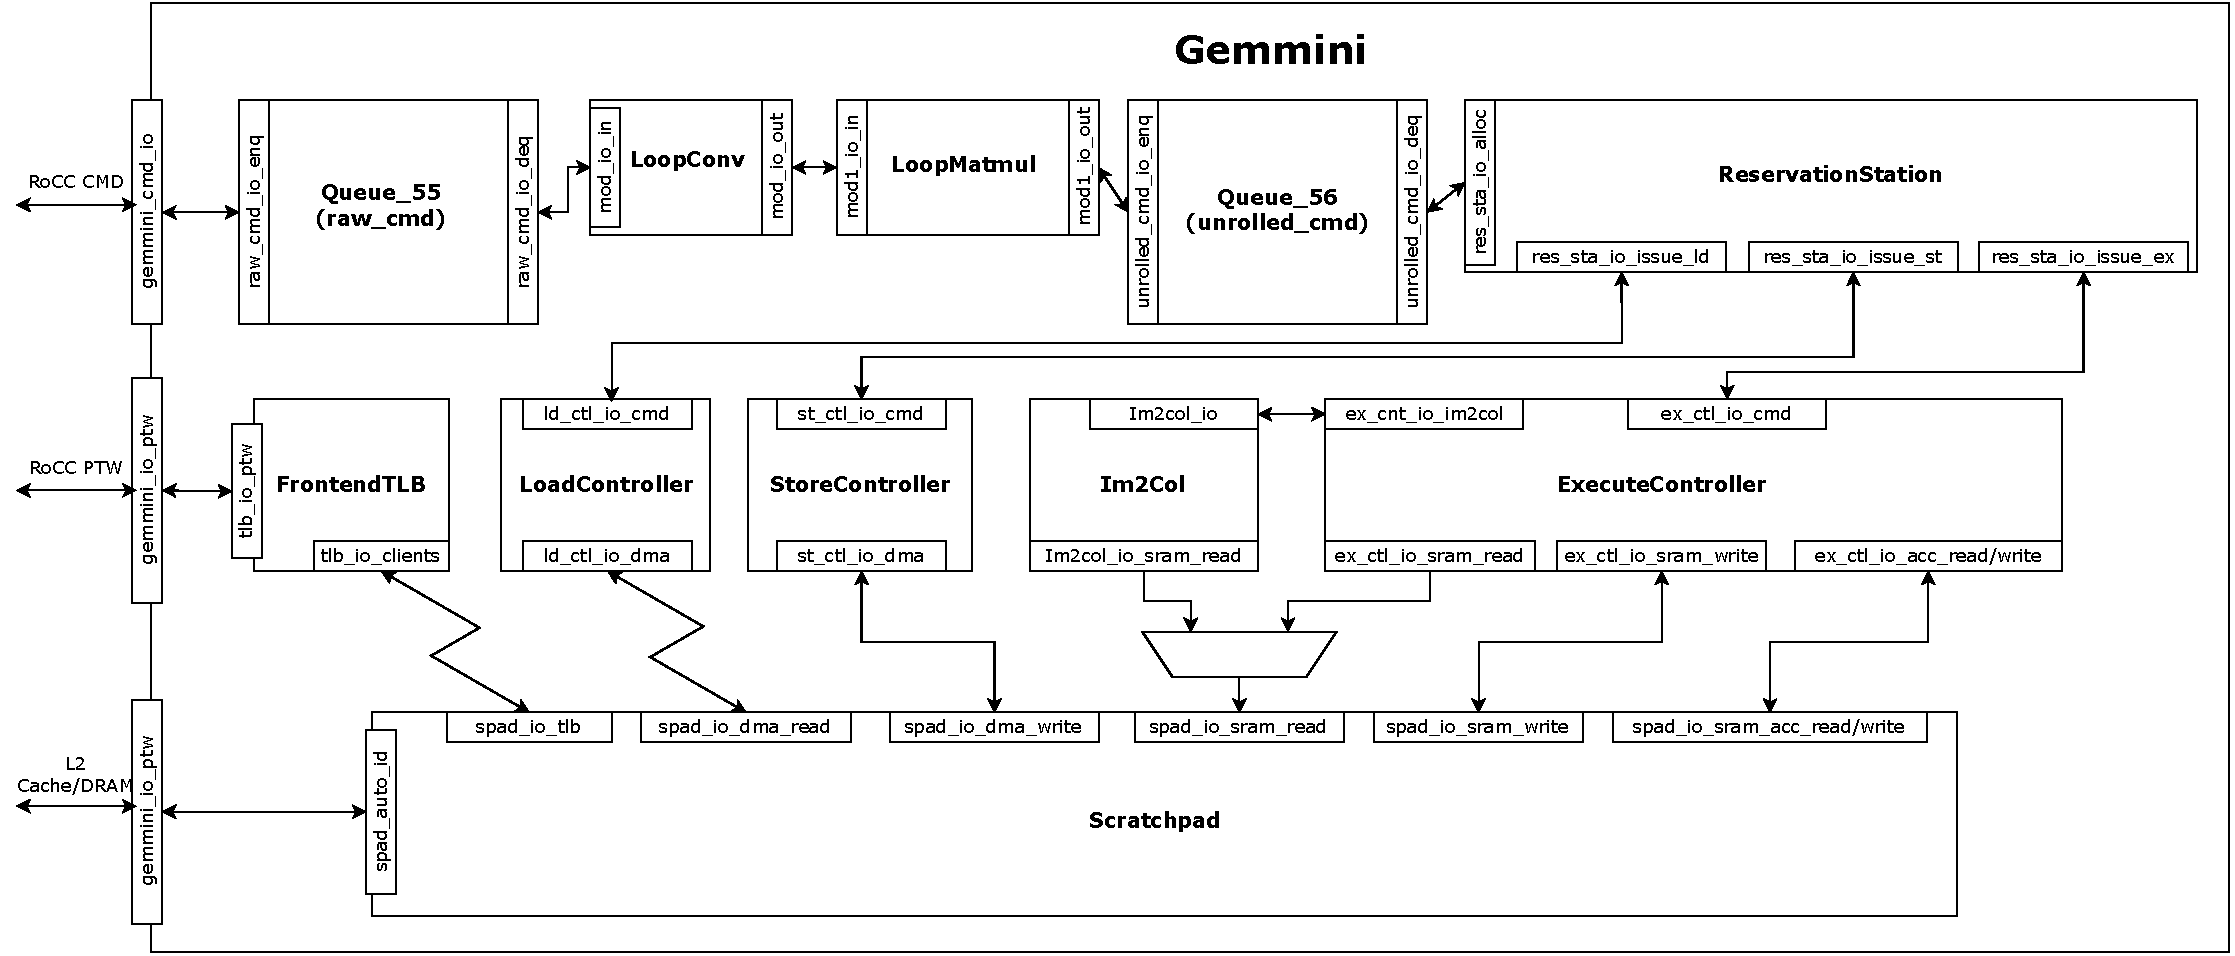
\includegraphics[width=\textwidth]{Gemmini_InternalOverview.pdf}
    \caption{Overview of the internal modules in the generated Gemmini hardware architecture, showing the flow of commands from the RoCC interface through various queues and controllers. Source: \cite{gookyi2023gemmini_case_study}.}
    \label{fig:gemmini_internal_modules}
\end{figure}

\subsection{Command Unrolling and Buffering}
The initial \texttt{RoCC} instructions received from the CPU are often "complex" commands that encapsulate entire loops (e.g., `loop\_matmul`). As shown in Figure~\ref{fig:command_unrollers}, modules like \texttt{LoopMatmul} and \texttt{LoopConv} are responsible for unrolling these high-level tasks into a stream of simpler, primitive micro-operations for loading, storing, and executing on tiled sub-matrices. These primitive commands are then buffered in a queue before being sent to a central dispatcher.

\begin{figure}[htbp]
    \centering
    \includegraphics[width=\textwidth]{_YOUR_IMAGE_PATH_/Sensors_Fig4.png}
    \caption{Gemmini's command unrolling modules (\texttt{LoopConv} and \texttt{LoopMatmul}), which translate high-level commands into a series of primitive operations. Source: \cite{gookyi2023gemmini_case_study}.}
    \label{fig:command_unrollers}
\end{figure}

\subsection{Reservation Station and Execution Control}
The stream of primitive commands is received by the \texttt{ReservationStation} module, which reorders and dispatches them to the appropriate back-end controller. The \texttt{ExecuteController} (Figure~\ref{fig:execute_controller}) manages the actual computation. It issues commands to the systolic array and orchestrates the movement of data between the scratchpad and the computational units. It also contains logic to manage optional units, such as the hardware \texttt{im2col} unit or data transposer.

\begin{figure}[htbp]
    \centering
    \includegraphics[width=\textwidth]{_YOUR_IMAGE_PATH_/Sensors_Fig6.png}
    \caption{The \texttt{ExecuteController} module and its associated SRAM control interfaces. Source: \cite{gookyi2023gemmini_case_study}.}
    \label{fig:execute_controller}
\end{figure}

\subsection{The Mesh and Scratchpad}
The \texttt{ExecuteController} ultimately controls the two lowest-level hardware blocks: the \texttt{Mesh} and the \texttt{Scratchpad}. The \texttt{Mesh} (Figure~\ref{fig:mesh_module}) is the direct hardware implementation of the systolic array, containing the grid of PEs. The \texttt{Scratchpad} (Figure~\ref{fig:scratchpad_module}) implements the on-chip memory, containing the SRAM banks and logic for interfacing with the DMA engine and the systolic array's accumulator.

\begin{figure}[htbp]
    \centering
    \includegraphics[width=0.7\textwidth]{_YOUR_IMAGE_PATH_/Sensors_Fig8.png}
    \caption{The \texttt{Mesh} module, which implements the systolic array of PEs and supports different dataflows (Output Stationary and Weight Stationary). Source: \cite{gookyi2023gemmini_case_study}.}
    \label{fig:mesh_module}
\end{figure}

\begin{figure}[htbp]
    \centering
    \includegraphics[width=\textwidth]{_YOUR_IMAGE_PATH_/Sensors_Fig9.png}
    \caption{The internal structure of the \texttt{Scratchpad} module, showing the various interfaces to the TLB, DMA, and internal memory banks. Source: \cite{gookyi2023gemmini_case_study}.}
    \label{fig:scratchpad_module}
\end{figure}

\section{The Multi-Level Programming Model}
\label{sec:gemmini_programming_model}

To cater to different user needs, from application developers to hardware architects, \texttt{Gemmini} supports a multi-level programming model. This stack provides layers of abstraction, allowing users to work at a level appropriate for their task, from direct hardware control to high-level framework integration.

\subsection{Low-Level: Gemmini ISA}
At the lowest level, \texttt{Gemmini} is controlled by its custom RoCC instruction set. These instructions are typically wrapped in C preprocessor macros for easier use from C/C++ code. The instruction set includes primitive commands like \texttt{mvin} (move data in), \texttt{mvout} (move data out), \texttt{preload} (load data into the PE array), and \texttt{compute}. It also features more "complex" instructions like \texttt{loop\_matmul} that abstract away the manual tiling and scheduling of primitive commands, offloading the loop control to hardware state machines \cite{Genc2022GemminiMLSys}.

\subsection{Mid-Level: Hand-Tuned C Library}
To abstract the complexities of direct ISA programming, \texttt{Gemmini} provides a C library (typically accessed via \texttt{gemmini.h}). This library offers functions for common DNN operations, such as \texttt{tiled\_matmul} and \texttt{tiled\_conv}. These functions implement optimized heuristics for loop tiling and data movement to maximize scratchpad utilization based on the specific hardware parameters of the generated \texttt{Gemmini} instance.

\subsection{High-Level: Compiler Support (Conceptual)}
The \texttt{Gemmini} ecosystem is designed to support higher-level compilation flows. This involves tools that can take DNN models described in standard frameworks like ONNX (Open Neural Network Exchange) and compile them down to \texttt{Gemmini} instructions, either by calling the mid-level C library or by directly generating low-level ISA calls. This further simplifies the deployment of DNNs on \texttt{Gemmini}-accelerated SoCs.

\section{Gemmini Configuration in This Thesis}
\label{sec:gemmini_configuration}

The \texttt{Gemmini} accelerator integrated into the SoC for this thesis is based on a specific configuration suitable for the target AI applications and FPGA resource constraints. Within the \texttt{Chipyard} framework, this configuration is defined in a \texttt{Scala} configuration file. 
\todo[inline]{Specify the key parameters for your Gemmini instance here. For example: The instance was configured with a 16x16 systolic array using 8-bit integer data types for inputs and weights, and a 32-bit integer accumulator. The scratchpad was configured with 256KB of capacity and the accumulator memory with 64KB. The Weight Stationary (WS) dataflow was selected, and the hardware \texttt{im2col} unit was included to offload this pre-processing step from the host CPU. These parameters were chosen to balance performance for target DNN workloads with the resource constraints of the target FPGA. The detailed performance implications of these choices will be explored in subsequent chapters.}

The integration follows the standard \texttt{RoCC} methodology provided by \texttt{Chipyard}, ensuring that \texttt{Gemmini} coexists with the \texttt{Rocket} Core, shares the system memory hierarchy, and can be programmed using custom RISC-V instructions dispatched to its \texttt{RoCC} slot.